%%% MATH COMMANDS %%%
\newcommand{\R}{\ensuremath{\mathbb{R}}}
\newcommand{\RNum}[1]{\uppercase\expandafter{\romannumeral #1\relax}}
\def\intavg{\,\ThisStyle{\ensurestackMath{%
    \stackinset{c}{0\LMpt}{c}{0\LMpt}{\SavedStyle-}{\SavedStyle\phantom{\int}}}%
    \setbox0=\hbox{$\SavedStyle\int\,$}\kern-\wd0}\int}
%%%%%%%%%%%%%%%%%%%%%

\documentclass[12pt]{artikel1}
\usepackage{scalerel}
\usepackage[usestackEOL]{stackengine}
\usepackage{pgfplots}
\pgfplotsset{compat=1.18}
\usepackage{amsmath}
\usepackage{amsthm}
\usepackage{tikz}
\usetikzlibrary{3d}
\usepackage[utf8]{inputenc}
\usepackage{graphicx}
\usepackage[english]{babel}
\usepackage[a4paper, margin=3cm]{geometry}
\usepackage[T1]{fontenc}
\sffamily
\usepackage{textpos}
\usepackage{amssymb}
\usepackage{listings}
\usepackage{eurosym}
\usepackage{ragged2e}
\usepackage{blindtext}
\usepackage{romannum}
\usepackage[
    backend=biber,
    style=apa,
  ]{biblatex}
\usepackage[most]{tcolorbox}
\addbibresource{PDE.bib}
\usepackage{hyperref}
\hypersetup{
    pdfpagemode=UseNone, 
    colorlinks=true,
    filecolor=blue,
    linkcolor=red,
    citecolor=black,
    urlcolor=blue
}
\DeclareAutoCiteCommand{textcite}{\textcite}{\textcites}
\ExecuteBibliographyOptions{autocite=textcite}
\linespread{1.25}
\DeclareMathOperator*{\argmax}{arg\,max}
\newtheorem{proposition}{Proposition}[section]
\newtheorem{theorem}{Theorem}[section]
\newtheorem{corollary}{Corollary}[theorem]
\newtheorem{lemma}[theorem]{Lemma}
\newtheorem{definition}{Definition}[section]

\begin{document}
\pagenumbering{arabic}
\begin{textblock*}{250mm}(0cm,-2cm)
\noindent Partial Differential Equations \RN{2}
\end{textblock*}
\begin{textblock*}{250mm}(.80\textwidth,-2cm)
\noindent Santeri Väätäjä
\end{textblock*}
\vspace*{-2cm}
\section*{Regularity of Elliptic Second Order Partial Differential Equations: Calder\'{o}n-Zygmund estimates}
\vspace*{-.5cm}
\line(1,0){10cm}
\vspace*{.5cm}

\noindent The regularity of solutions to second-order elliptic differential equations refers to the smoothness or differentiability of these solutions. This concept is crucial in the theory of partial differential equations (PDEs) as it determines how well-behaved the solutions are and whether they satisfy the equation in a classical or weak sense.

One line of attack that can be taken in the case of second-order elliptic PDEs, and especially in this case with the Laplacian equation, is to examine if the principle that \cite{Fern_ndez_Real_2022} calls ``$u$ is two derivatives more regular than $f$''. The results regarding this phenomenon can be divided into two main results

\begin{enumerate}
    \item \textit{Schauder estimates:} If $f\in C^{0,\alpha}$ then $u\in C^{2,\alpha}$, for $\alpha\in(0,1)$, or more generally if $f\in C^{k,\alpha}$ then $u\in C^{k+2,\alpha}$.
    \item \textit{Calder\'{o}n-Zygmund estimates:} If $f\in L^p$ then $u\in W^{2,p}$ for $p\in(1,\infty)$.
\end{enumerate}

\noindent From these two, the first one is shown in the lecture notes \cite{covi}, so with interest in expanding the regularity theory of upgrading the weak solutions of the Laplace equation, I will be concentrating on the second item in the list; Calder\'{o}n-Zygmund estimates.

These, unlike Schauder estimates, consider functions in $L^p$-space, so unlike in the first case, we lose the pointwise control of the functions.  Schauder estimates are concerned with the regularity of solutions at each individual point in the domain, requiring that the given data be Hölder continuous. This means that the data must exhibit a certain level of smoothness and continuity pointwise, allowing for precise control over the behavior of the solution at every location. In contrast, Calderón-Zygmund estimates deal with functions that are integrable but may lack pointwise smoothness. These estimates operate within $L^p$-spaces, where the focus is on the overall integrability of the functions rather than their pointwise behavior. As a result, Calderón-Zygmund estimates provide regularity results based on the average properties of the functions, making them applicable even when the data is less regular but still integrable.

I will be restricting the forthcoming analysis to consider only the case where the domain of the Laplacian is assumed to be $\Omega=B_1$, following the analysis done in \cite{covi,Fern_ndez_Real_2022} and \cite{sanpera} which I will be be primarily following on the proofs for Calder\'{o}n-Zygmund estimates. It would be possible to extend the analysis to cover a broader family of domains than the unit ball, but the restriction is made in order to restrict the complexity of the analysis.

\subsection*{Formalization of the Problem}

The problem of establishing some regularity starts by having the Laplacian

\begin{gather}\label{eq:laplacian}
    \begin{cases}
        \Delta u=f,\,x\in B_1 \\
        u=g,\,x\in\partial B_1
    \end{cases}
\end{gather}

\noindent and in the case of Calder\'{o}n-Zygmund estimates we further assume that $f\in L^{p}(B_1)$. Then the estimates give that if $u$ is a weak solution to the problem \ref{eq:laplacian}, then $D^2u\in L^p$ for $p\in (1,\infty)$. The definition of a weak solution is given as follows:

\begin{definition}\label{def:weak}
    A function $u$ is a weak solution of \ref{eq:laplacian} if $u\in H^1(\Omega)$, $u|_{\partial\Omega}=g$ and 
    \begin{gather*}
        \int_\Omega\nabla u\nabla v=\int_\Omega fv
    \end{gather*}
    for all $v\in H^1(\Omega)$ such that $v=0$ in $\partial\Omega$.
\end{definition}

\noindent The proof for this can be treated differently for some specific values of $p$, most notably for $p=2$, which allows a more straightforward proof. It is also noteworthy that the values $1$ and $\infty$ are excluded from the formulation. In these cases, the inclusion of the solution to the $L^p$-space cannot be guaranteed. However, there exist some versions of these estimates that can be given in the case of $L^\infty$. These results are introduced in \cite{sanpera}. This requires introducing new concepts for the function space in which the result applies, namely something called a BMO space. The BMO space is a concept that shares similarities with both Hölder and Sobolev spaces. I will not be concentrating on these estimates, but rather stick with the original bounds for $p$.

To get a better idea of why the estimates hold only for such values of $p$ \cite{Fern_ndez_Real_2022} presents some examples of harmonic functions that exhibit the behavior. In the case for $p=1$, taking the mollified Dirac delta to be the example $f_\epsilon(x)=\epsilon^{-n}\eta(\frac{x}{\epsilon})$ so $f_\epsilon\in C^{\infty}$ and it converges towards the fundamental solution as $\epsilon\rightarrow0$, but that does not belong in the $W^{2,1}$.

\begin{figure}[h]
    \centering
    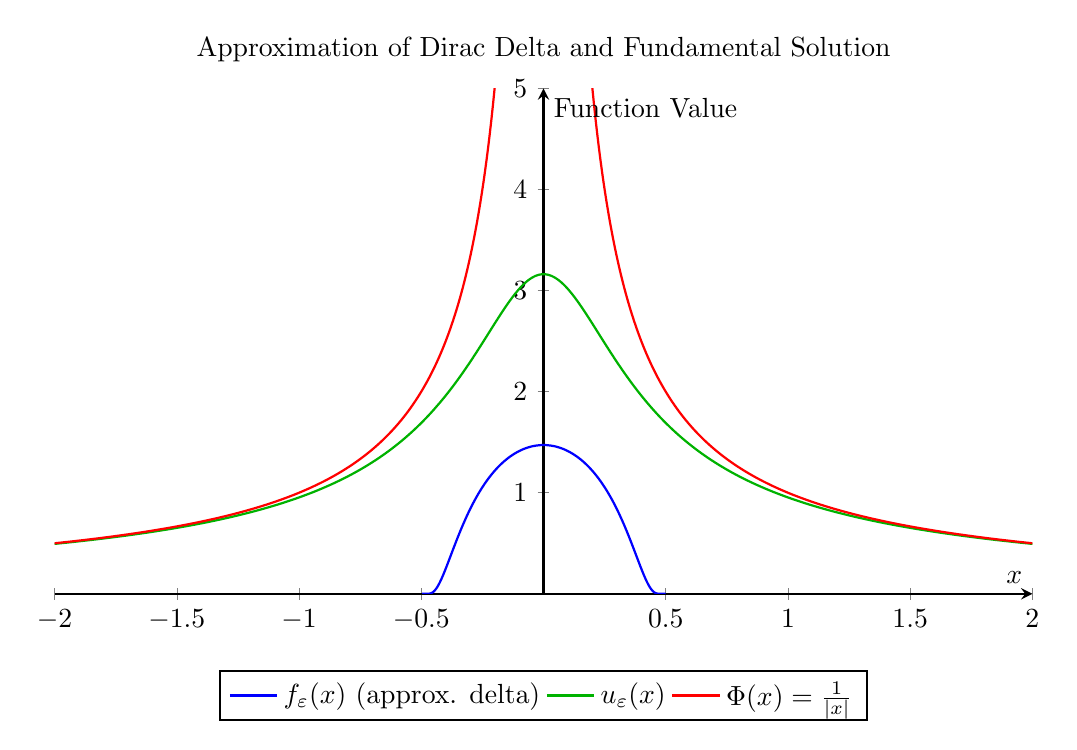
\begin{tikzpicture}
\begin{axis}[
    title={Approximation of Dirac Delta and Fundamental Solution},
    axis lines=middle,
    xlabel={$x$},
    ylabel={Function Value},
    legend style={at={(0.5,-0.15)}, anchor=north, legend columns=3},
    xmin=-2, xmax=2,
    ymin=0, ymax=5,
    samples=300,
    domain=-2:2,
    width=14cm,
    height=8cm,
    thick,
]

% Mollifier f_epsilon (bump function)
\addplot[blue, thick, domain=-0.5:0.5] {4 * exp(-1/(1 - (x/0.5)^2))};
\addlegendentry{$f_\varepsilon(x)$ (approx. delta)}

% Solution u_epsilon (smoothed 1/|x| version)
\addplot[green!70!black, thick, domain=-2:2] {1 / sqrt(x^2 + 0.1)};
\addlegendentry{$u_\varepsilon(x)$}

% Fundamental solution 1/|x|
\addplot[red, thick, domain=0.05:2] {1/x};
\addplot[red, thick, domain=-2:-0.05] {-1/x}; % Symmetric for absolute value
\addlegendentry{$\Phi(x) = \frac{1}{|x|}$}

\end{axis}
\end{tikzpicture}
    \caption{Caption}
    \label{fig:failure}
\end{figure}

\subsection*{Regularity in $L^p$}

Now we can proceed to stating the theorem and then proving it. As suggested, the theorem states that the solution $u$ is two derivatives more regular compared than the function $f$. In the context of $L^p$ this means that for $f\in L^p$ we would need the solution to belong in $W^{2,p}$. The next theorem states the exact formulation of this claim.

\begin{theorem}\label{thm:main}
    Let $u\in H^1(B_1)$ be a weak solution to
    \begin{equation*}
        \Delta u=f\text{ in }B_1,
    \end{equation*}
    with $f\in L^p(B_1)$. Then u is $W^{2,p}$ inside $B_1$ and the following estimate holds
    \begin{equation*}
        \int_{B_1}|D^2u|^p\leq C\left(\int_{B_2}|u|^p+\int_{B_2}|f|^p\right)
    \end{equation*}
\end{theorem}

Let's first establish one auxiliary result for $L^p$-spaces that will be needed to begin the proof for the main result. 

\begin{proposition}
    Let $(X,\mathcal{F},\mu)$ be a measure space. Let $\nu$ be a Borel measure on $[0,\infty)$ and $f\in\mathcal{M}_+$. For $\lambda,t\geq0$, set
    \begin{equation*}
        \phi(t)=\int_0^td\nu(s),\, u(\lambda)=\mu\{f>\lambda\}
    \end{equation*}
    then
    \begin{equation*}
        \int \phi(f(x))=\int_0^\infty u(\lambda)d\nu(\lambda)
    \end{equation*}
\end{proposition}
\begin{proof}
    \begin{align*}
        \int_0^\infty u(\lambda)d\nu(\lambda)&=\int\left(\int\chi_{\{f>\lambda\}}d\mu(x)\right)d\nu(\lambda) \\
        &= \int\left(\int\chi_{\{f>\lambda\}}d\nu(\lambda)\right)d\mu(x) \\
        &=\int\left(\int_0^{f(x)}d\nu(\lambda)\right)d\mu(x) \\
        &=\int\phi(f(x))d\mu(x)
    \end{align*}
\end{proof}

\noindent From this, we can yield a corollary that gives a way to represent the $L^p$ norm with respect to the sets on which the function gets values that are larger than a given constant.

\begin{corollary}
    \begin{equation*}
        \int|f(x)|^pd\mu(x)=p\int_0^\infty u(\lambda)\lambda^{p-1}d\lambda
    \end{equation*}
\end{corollary}
\begin{proof}
    Let $\phi(t)=t^p$ and $d\nu(t)=pt^{p-1}$, then the integral is acquired by the change of variables.
\end{proof}

\noindent This implies that for the norm to be finite, measures of sets $\{x\in\Omega|\,|u(x)|>\lambda\}$ have to shrink as the $\lambda\rightarrow\infty$. From now on, I will denote the normal Lebesgue measure as $|\cdot|$.

Now we would like to use this result to prove a tail estimate for the norms of $u$ and $f$ that would lead us to a similar inequality given in the theorem \ref{thm:main}.

\clearpage
\printbibliography

\end{document}
